\documentclass[1p]{elsarticle_modified}
%\bibliographystyle{elsarticle-num}

%\usepackage[colorlinks]{hyperref}
%\usepackage{abbrmath_seonhwa} %\Abb, \Ascr, \Acal ,\Abf, \Afrak
\usepackage{amsfonts}
\usepackage{amssymb}
\usepackage{amsmath}
\usepackage{amsthm}
\usepackage{scalefnt}
\usepackage{amsbsy}
\usepackage{kotex}
\usepackage{caption}
\usepackage{subfig}
\usepackage{color}
\usepackage{graphicx}
\usepackage{xcolor} %% white, black, red, green, blue, cyan, magenta, yellow
\usepackage{float}
\usepackage{setspace}
\usepackage{hyperref}

\usepackage{tikz}
\usetikzlibrary{arrows}

\usepackage{multirow}
\usepackage{array} % fixed length table
\usepackage{hhline}

%%%%%%%%%%%%%%%%%%%%%
\makeatletter
\renewcommand*\env@matrix[1][\arraystretch]{%
	\edef\arraystretch{#1}%
	\hskip -\arraycolsep
	\let\@ifnextchar\new@ifnextchar
	\array{*\c@MaxMatrixCols c}}
\makeatother %https://tex.stackexchange.com/questions/14071/how-can-i-increase-the-line-spacing-in-a-matrix
%%%%%%%%%%%%%%%

\usepackage[normalem]{ulem}

\newcommand{\msout}[1]{\ifmmode\text{\sout{\ensuremath{#1}}}\else\sout{#1}\fi}
%SOURCE: \msout is \stkout macro in https://tex.stackexchange.com/questions/20609/strikeout-in-math-mode

\newcommand{\cancel}[1]{
	\ifmmode
	{\color{red}\msout{#1}}
	\else
	{\color{red}\sout{#1}}
	\fi
}

\newcommand{\add}[1]{
	{\color{blue}\uwave{#1}}
}

\newcommand{\replace}[2]{
	\ifmmode
	{\color{red}\msout{#1}}{\color{blue}\uwave{#2}}
	\else
	{\color{red}\sout{#1}}{\color{blue}\uwave{#2}}
	\fi
}

\newcommand{\Sol}{\mathcal{S}} %segment
\newcommand{\D}{D} %diagram
\newcommand{\A}{\mathcal{A}} %arc


%%%%%%%%%%%%%%%%%%%%%%%%%%%%%5 test

\def\sl{\operatorname{\textup{SL}}(2,\Cbb)}
\def\psl{\operatorname{\textup{PSL}}(2,\Cbb)}
\def\quan{\mkern 1mu \triangleright \mkern 1mu}

\theoremstyle{definition}
\newtheorem{thm}{Theorem}[section]
\newtheorem{prop}[thm]{Proposition}
\newtheorem{lem}[thm]{Lemma}
\newtheorem{ques}[thm]{Question}
\newtheorem{cor}[thm]{Corollary}
\newtheorem{defn}[thm]{Definition}
\newtheorem{exam}[thm]{Example}
\newtheorem{rmk}[thm]{Remark}
\newtheorem{alg}[thm]{Algorithm}

\newcommand{\I}{\sqrt{-1}}
\begin{document}

%\begin{frontmatter}
%
%\title{Boundary parabolic representations of knots up to 8 crossings}
%
%%% Group authors per affiliation:
%\author{Yunhi Cho} 
%\address{Department of Mathematics, University of Seoul, Seoul, Korea}
%\ead{yhcho@uos.ac.kr}
%
%
%\author{Seonhwa Kim} %\fnref{s_kim}}
%\address{Center for Geometry and Physics, Institute for Basic Science, Pohang, 37673, Korea}
%\ead{ryeona17@ibs.re.kr}
%
%\author{Hyuk Kim}
%\address{Department of Mathematical Sciences, Seoul National University, Seoul 08826, Korea}
%\ead{hyukkim@snu.ac.kr}
%
%\author{Seokbeom Yoon}
%\address{Department of Mathematical Sciences, Seoul National University, Seoul, 08826,  Korea}
%\ead{sbyoon15@snu.ac.kr}
%
%\begin{abstract}
%We find all boundary parabolic representation of knots up to 8 crossings.
%
%\end{abstract}
%\begin{keyword}
%    \MSC[2010] 57M25 
%\end{keyword}
%
%\end{frontmatter}

%\linenumbers
%\tableofcontents
%
\newcommand\colored[1]{\textcolor{white}{\rule[-0.35ex]{0.8em}{1.4ex}}\kern-0.8em\color{red} #1}%
%\newcommand\colored[1]{\textcolor{white}{ #1}\kern-2.17ex	\textcolor{white}{ #1}\kern-1.81ex	\textcolor{white}{ #1}\kern-2.15ex\color{red}#1	}

{\Large $\underline{12a_{0153}~(K12a_{0153})}$}

\setlength{\tabcolsep}{10pt}
\renewcommand{\arraystretch}{1.6}
\vspace{1cm}\begin{tabular}{m{100pt}>{\centering\arraybackslash}m{274pt}}
\multirow{5}{120pt}{
	\centering
	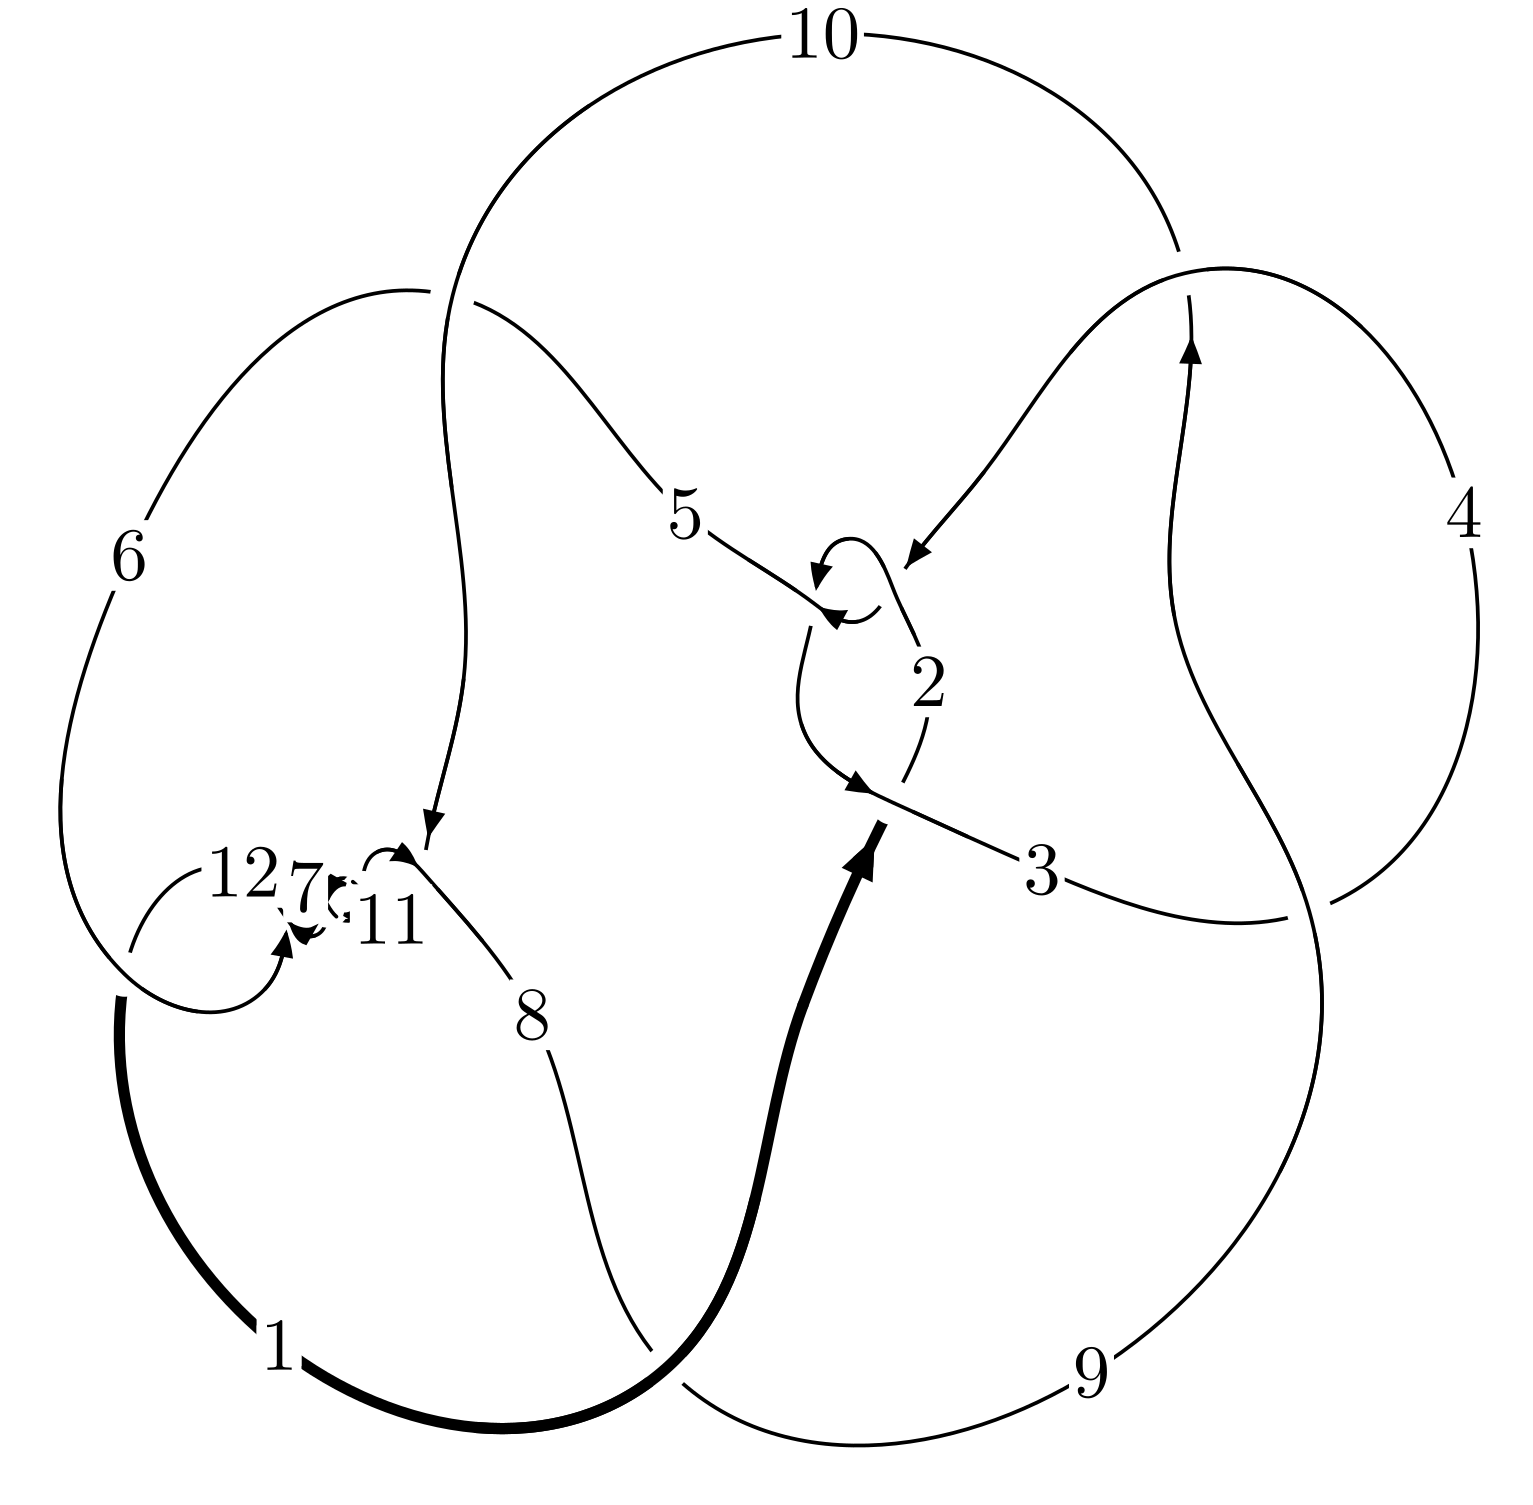
\includegraphics[width=112pt]{../../../GIT/diagram.site/Diagrams/png/954_12a_0153.png}\\
\ \ \ A knot diagram\footnotemark}&
\allowdisplaybreaks
\textbf{Linearized knot diagam} \\
\cline{2-2}
 &
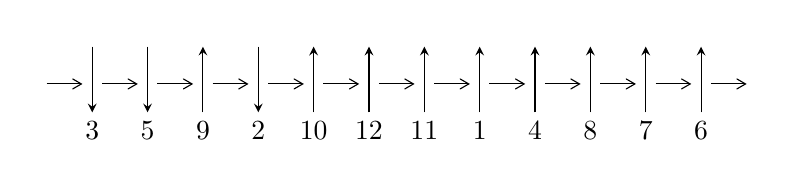
\begin{tikzpicture}[x=20pt, y=17pt]
	% nodes
	\node (C0) at (0, 0) {};
	\node (C1) at (1, 0) {};
	\node (C1U) at (1, +1) {};
	\node (C1D) at (1, -1) {3};

	\node (C2) at (2, 0) {};
	\node (C2U) at (2, +1) {};
	\node (C2D) at (2, -1) {5};

	\node (C3) at (3, 0) {};
	\node (C3U) at (3, +1) {};
	\node (C3D) at (3, -1) {9};

	\node (C4) at (4, 0) {};
	\node (C4U) at (4, +1) {};
	\node (C4D) at (4, -1) {2};

	\node (C5) at (5, 0) {};
	\node (C5U) at (5, +1) {};
	\node (C5D) at (5, -1) {10};

	\node (C6) at (6, 0) {};
	\node (C6U) at (6, +1) {};
	\node (C6D) at (6, -1) {12};

	\node (C7) at (7, 0) {};
	\node (C7U) at (7, +1) {};
	\node (C7D) at (7, -1) {11};

	\node (C8) at (8, 0) {};
	\node (C8U) at (8, +1) {};
	\node (C8D) at (8, -1) {1};

	\node (C9) at (9, 0) {};
	\node (C9U) at (9, +1) {};
	\node (C9D) at (9, -1) {4};

	\node (C10) at (10, 0) {};
	\node (C10U) at (10, +1) {};
	\node (C10D) at (10, -1) {8};

	\node (C11) at (11, 0) {};
	\node (C11U) at (11, +1) {};
	\node (C11D) at (11, -1) {7};

	\node (C12) at (12, 0) {};
	\node (C12U) at (12, +1) {};
	\node (C12D) at (12, -1) {6};
	\node (C13) at (13, 0) {};

	% arrows
	\draw[->,>={angle 60}]
	(C0) edge (C1) (C1) edge (C2) (C2) edge (C3) (C3) edge (C4) (C4) edge (C5) (C5) edge (C6) (C6) edge (C7) (C7) edge (C8) (C8) edge (C9) (C9) edge (C10) (C10) edge (C11) (C11) edge (C12) (C12) edge (C13) ;	\draw[->,>=stealth]
	(C1U) edge (C1D) (C2U) edge (C2D) (C3D) edge (C3U) (C4U) edge (C4D) (C5D) edge (C5U) (C6D) edge (C6U) (C7D) edge (C7U) (C8D) edge (C8U) (C9D) edge (C9U) (C10D) edge (C10U) (C11D) edge (C11U) (C12D) edge (C12U) ;
	\end{tikzpicture} \\
\hhline{~~} \\& 
\textbf{Solving Sequence} \\ \cline{2-2} 
 &
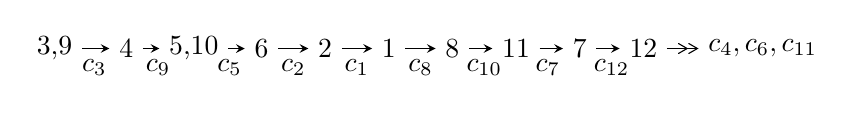
\begin{tikzpicture}[x=23pt, y=7pt]
	% node
	\node (A0) at (-1/8, 0) {3,9};
	\node (A1) at (1, 0) {4};
	\node (A2) at (33/16, 0) {5,10};
	\node (A3) at (25/8, 0) {6};
	\node (A4) at (33/8, 0) {2};
	\node (A5) at (41/8, 0) {1};
	\node (A6) at (49/8, 0) {8};
	\node (A7) at (57/8, 0) {11};
	\node (A8) at (65/8, 0) {7};
	\node (A9) at (73/8, 0) {12};
	\node (C1) at (1/2, -1) {$c_{3}$};
	\node (C2) at (3/2, -1) {$c_{9}$};
	\node (C3) at (21/8, -1) {$c_{5}$};
	\node (C4) at (29/8, -1) {$c_{2}$};
	\node (C5) at (37/8, -1) {$c_{1}$};
	\node (C6) at (45/8, -1) {$c_{8}$};
	\node (C7) at (53/8, -1) {$c_{10}$};
	\node (C8) at (61/8, -1) {$c_{7}$};
	\node (C9) at (69/8, -1) {$c_{12}$};
	\node (A10) at (11, 0) {$c_{4},c_{6},c_{11}$};

	% edge
	\draw[->,>=stealth]	
	(A0) edge (A1) (A1) edge (A2) (A2) edge (A3) (A3) edge (A4) (A4) edge (A5) (A5) edge (A6) (A6) edge (A7) (A7) edge (A8) (A8) edge (A9) ;
	\draw[->>,>={angle 60}]	
	(A9) edge (A10);
\end{tikzpicture} \\ 

\end{tabular} \\

\footnotetext{
The image of knot diagram is generated by the software ``\textbf{Draw programme}" developed by Andrew Bartholomew(\url{http://www.layer8.co.uk/maths/draw/index.htm\#Running-draw}), where we modified some parts for our purpose(\url{https://github.com/CATsTAILs/LinksPainter}).
}\phantom \\ \newline 
\centering \textbf{Ideals for irreducible components\footnotemark of $X_{\text{par}}$} 
 
\begin{align*}
I^u_{1}&=\langle 
5.60722\times10^{81} u^{57}+1.67247\times10^{81} u^{56}+\cdots+2.33772\times10^{82} b+1.81103\times10^{83},\\
\phantom{I^u_{1}}&\phantom{= \langle  }7.27818\times10^{82} u^{57}+4.91560\times10^{82} u^{56}+\cdots+1.87018\times10^{83} a+1.91879\times10^{84},\;u^{58}+u^{57}+\cdots+64 u+32\rangle \\
\\
I^v_{1}&=\langle 
a,\;b-1,\;v^5- v^4+v^2+v-1\rangle \\
\end{align*}
\raggedright * 2 irreducible components of $\dim_{\mathbb{C}}=0$, with total 63 representations.\\
\footnotetext{All coefficients of polynomials are rational numbers. But the coefficients are sometimes approximated in decimal forms when there is not enough margin.}
\newpage
\renewcommand{\arraystretch}{1}
\centering \section*{I. $I^u_{1}= \langle 5.61\times10^{81} u^{57}+1.67\times10^{81} u^{56}+\cdots+2.34\times10^{82} b+1.81\times10^{83},\;7.28\times10^{82} u^{57}+4.92\times10^{82} u^{56}+\cdots+1.87\times10^{83} a+1.92\times10^{84},\;u^{58}+u^{57}+\cdots+64 u+32 \rangle$}
\flushleft \textbf{(i) Arc colorings}\\
\begin{tabular}{m{7pt} m{180pt} m{7pt} m{180pt} }
\flushright $a_{3}=$&$\begin{pmatrix}1\\0\end{pmatrix}$ \\
\flushright $a_{9}=$&$\begin{pmatrix}0\\u\end{pmatrix}$ \\
\flushright $a_{4}=$&$\begin{pmatrix}1\\- u^2\end{pmatrix}$ \\
\flushright $a_{5}=$&$\begin{pmatrix}-0.389171 u^{57}-0.262841 u^{56}+\cdots+4.54781 u-10.2600\\-0.239859 u^{57}-0.0715429 u^{56}+\cdots-7.02146 u-7.74698\end{pmatrix}$ \\
\flushright $a_{10}=$&$\begin{pmatrix}u\\- u^3+u\end{pmatrix}$ \\
\flushright $a_{6}=$&$\begin{pmatrix}-0.522817 u^{57}-0.268126 u^{56}+\cdots-1.68093 u-13.8759\\-0.207902 u^{57}-0.0373370 u^{56}+\cdots-9.31175 u-7.25535\end{pmatrix}$ \\
\flushright $a_{2}=$&$\begin{pmatrix}-0.389171 u^{57}-0.262841 u^{56}+\cdots+4.54781 u-10.2600\\0.420518 u^{57}+0.181191 u^{56}+\cdots+2.65309 u+11.7895\end{pmatrix}$ \\
\flushright $a_{1}=$&$\begin{pmatrix}0.0313472 u^{57}-0.0816505 u^{56}+\cdots+7.20090 u+1.52957\\0.420518 u^{57}+0.181191 u^{56}+\cdots+2.65309 u+11.7895\end{pmatrix}$ \\
\flushright $a_{8}=$&$\begin{pmatrix}-0.713059 u^{57}+0.0359583 u^{56}+\cdots-41.8715 u-42.2736\\-0.0618638 u^{57}+0.0517051 u^{56}+\cdots-0.420514 u+0.205394\end{pmatrix}$ \\
\flushright $a_{11}=$&$\begin{pmatrix}0.427906 u^{57}+0.0462409 u^{56}+\cdots+18.0771 u+11.5849\\-0.749808 u^{57}+0.0101401 u^{56}+\cdots-32.6805 u-32.2330\end{pmatrix}$ \\
\flushright $a_{7}=$&$\begin{pmatrix}0.393422 u^{57}+0.397378 u^{56}+\cdots-1.00737 u+23.9064\\-0.558340 u^{57}-0.192853 u^{56}+\cdots-13.8407 u-26.9810\end{pmatrix}$ \\
\flushright $a_{12}=$&$\begin{pmatrix}0.460418 u^{57}+0.147034 u^{56}+\cdots+20.1920 u+18.9774\\-0.416036 u^{57}-0.145859 u^{56}+\cdots-7.89835 u-13.2725\end{pmatrix}$\\&\end{tabular}
\flushleft \textbf{(ii) Obstruction class $= -1$}\\~\\
\flushleft \textbf{(iii) Cusp Shapes $= -2.02102 u^{57}-0.114366 u^{56}+\cdots-107.539 u-65.1509$}\\~\\
\newpage\renewcommand{\arraystretch}{1}
\flushleft \textbf{(iv) u-Polynomials at the component}\newline \\
\begin{tabular}{m{50pt}|m{274pt}}
Crossings & \hspace{64pt}u-Polynomials at each crossing \\
\hline $$\begin{aligned}c_{1}\end{aligned}$$&$\begin{aligned}
&u^{58}+26 u^{57}+\cdots+36 u+1
\end{aligned}$\\
\hline $$\begin{aligned}c_{2},c_{4}\end{aligned}$$&$\begin{aligned}
&u^{58}-6 u^{57}+\cdots+12 u-1
\end{aligned}$\\
\hline $$\begin{aligned}c_{3},c_{9}\end{aligned}$$&$\begin{aligned}
&u^{58}- u^{57}+\cdots-64 u+32
\end{aligned}$\\
\hline $$\begin{aligned}c_{5},c_{8}\end{aligned}$$&$\begin{aligned}
&u^{58}+2 u^{57}+\cdots-1314 u-445
\end{aligned}$\\
\hline $$\begin{aligned}c_{6},c_{7},c_{10}\\c_{11},c_{12}\end{aligned}$$&$\begin{aligned}
&u^{58}+2 u^{57}+\cdots-2 u-1
\end{aligned}$\\
\hline
\end{tabular}\\~\\
\newpage\renewcommand{\arraystretch}{1}
\flushleft \textbf{(v) Riley Polynomials at the component}\newline \\
\begin{tabular}{m{50pt}|m{274pt}}
Crossings & \hspace{64pt}Riley Polynomials at each crossing \\
\hline $$\begin{aligned}c_{1}\end{aligned}$$&$\begin{aligned}
&y^{58}+18 y^{57}+\cdots-1608 y+1
\end{aligned}$\\
\hline $$\begin{aligned}c_{2},c_{4}\end{aligned}$$&$\begin{aligned}
&y^{58}-26 y^{57}+\cdots-36 y+1
\end{aligned}$\\
\hline $$\begin{aligned}c_{3},c_{9}\end{aligned}$$&$\begin{aligned}
&y^{58}-33 y^{57}+\cdots-19968 y+1024
\end{aligned}$\\
\hline $$\begin{aligned}c_{5},c_{8}\end{aligned}$$&$\begin{aligned}
&y^{58}-38 y^{57}+\cdots+2799054 y+198025
\end{aligned}$\\
\hline $$\begin{aligned}c_{6},c_{7},c_{10}\\c_{11},c_{12}\end{aligned}$$&$\begin{aligned}
&y^{58}+74 y^{57}+\cdots+6 y+1
\end{aligned}$\\
\hline
\end{tabular}\\~\\
\newpage\flushleft \textbf{(vi) Complex Volumes and Cusp Shapes}
$$\begin{array}{c|c|c}  
\text{Solutions to }I^u_{1}& \I (\text{vol} + \sqrt{-1}CS) & \text{Cusp shape}\\
 \hline 
\begin{aligned}
u &= -0.988918 + 0.213289 I \\
a &= \phantom{-}0.430565 + 0.018643 I \\
b &= \phantom{-}1.318190 - 0.100375 I\end{aligned}
 & -11.06150 - 4.52126 I & \phantom{-}2.64115 + 3.57478 I \\ \hline\begin{aligned}
u &= -0.988918 - 0.213289 I \\
a &= \phantom{-}0.430565 - 0.018643 I \\
b &= \phantom{-}1.318190 + 0.100375 I\end{aligned}
 & -11.06150 + 4.52126 I & \phantom{-}2.64115 - 3.57478 I \\ \hline\begin{aligned}
u &= -1.012520 + 0.149144 I \\
a &= \phantom{-}0.62352 + 1.58705 I \\
b &= -0.785549 - 0.545845 I\end{aligned}
 & \phantom{-}1.31063 - 0.82722 I & \phantom{-}9.15613 - 0.70745 I \\ \hline\begin{aligned}
u &= -1.012520 - 0.149144 I \\
a &= \phantom{-}0.62352 - 1.58705 I \\
b &= -0.785549 + 0.545845 I\end{aligned}
 & \phantom{-}1.31063 + 0.82722 I & \phantom{-}9.15613 + 0.70745 I \\ \hline\begin{aligned}
u &= \phantom{-}0.670998 + 0.708770 I \\
a &= \phantom{-}0.455472 - 0.072472 I \\
b &= \phantom{-}1.141310 + 0.340713 I\end{aligned}
 & -14.4352 - 1.2271 I & -2.32982 + 0.23811 I \\ \hline\begin{aligned}
u &= \phantom{-}0.670998 - 0.708770 I \\
a &= \phantom{-}0.455472 + 0.072472 I \\
b &= \phantom{-}1.141310 - 0.340713 I\end{aligned}
 & -14.4352 + 1.2271 I & -2.32982 - 0.23811 I \\ \hline\begin{aligned}
u &= \phantom{-}0.120330 + 1.017630 I \\
a &= \phantom{-}0.516133 - 0.162101 I \\
b &= \phantom{-}0.763532 + 0.553870 I\end{aligned}
 & -0.454989 + 0.856173 I & \phantom{-}4.39334 - 1.34405 I \\ \hline\begin{aligned}
u &= \phantom{-}0.120330 - 1.017630 I \\
a &= \phantom{-}0.516133 + 0.162101 I \\
b &= \phantom{-}0.763532 - 0.553870 I\end{aligned}
 & -0.454989 - 0.856173 I & \phantom{-}4.39334 + 1.34405 I \\ \hline\begin{aligned}
u &= -0.023513 + 1.056290 I \\
a &= \phantom{-}0.524037 + 0.186326 I \\
b &= \phantom{-}0.694092 - 0.602349 I\end{aligned}
 & -9.08024 - 2.35274 I & \phantom{-}2.89470 - 0.08369 I \\ \hline\begin{aligned}
u &= -0.023513 - 1.056290 I \\
a &= \phantom{-}0.524037 - 0.186326 I \\
b &= \phantom{-}0.694092 + 0.602349 I\end{aligned}
 & -9.08024 + 2.35274 I & \phantom{-}2.89470 + 0.08369 I\\
 \hline 
 \end{array}$$\newpage$$\begin{array}{c|c|c}  
\text{Solutions to }I^u_{1}& \I (\text{vol} + \sqrt{-1}CS) & \text{Cusp shape}\\
 \hline 
\begin{aligned}
u &= \phantom{-}0.926509 + 0.140364 I \\
a &= \phantom{-}0.436398 - 0.012440 I \\
b &= \phantom{-}1.289630 + 0.065266 I\end{aligned}
 & -2.19660 + 2.97198 I & \phantom{-}4.77337 - 5.16018 I \\ \hline\begin{aligned}
u &= \phantom{-}0.926509 - 0.140364 I \\
a &= \phantom{-}0.436398 + 0.012440 I \\
b &= \phantom{-}1.289630 - 0.065266 I\end{aligned}
 & -2.19660 - 2.97198 I & \phantom{-}4.77337 + 5.16018 I \\ \hline\begin{aligned}
u &= -0.229073 + 1.043540 I \\
a &= \phantom{-}0.495133 + 0.149970 I \\
b &= \phantom{-}0.849943 - 0.560327 I\end{aligned}
 & \phantom{-}1.83802 + 2.24390 I & \phantom{-}9.07567 - 3.44705 I \\ \hline\begin{aligned}
u &= -0.229073 - 1.043540 I \\
a &= \phantom{-}0.495133 - 0.149970 I \\
b &= \phantom{-}0.849943 + 0.560327 I\end{aligned}
 & \phantom{-}1.83802 - 2.24390 I & \phantom{-}9.07567 + 3.44705 I \\ \hline\begin{aligned}
u &= -0.898579\phantom{ +0.000000I} \\
a &= \phantom{-}0.439075\phantom{ +0.000000I} \\
b &= \phantom{-}1.27751\phantom{ +0.000000I}\end{aligned}
 & \phantom{-}0.376807\phantom{ +0.000000I} & \phantom{-}11.1020\phantom{ +0.000000I} \\ \hline\begin{aligned}
u &= \phantom{-}0.970754 + 0.521236 I \\
a &= -0.18922 - 2.00022 I \\
b &= -1.046870 + 0.495511 I\end{aligned}
 & -13.4454 + 5.9801 I & \phantom{-0.000000 } 0. - 6.24129 I \\ \hline\begin{aligned}
u &= \phantom{-}0.970754 - 0.521236 I \\
a &= -0.18922 + 2.00022 I \\
b &= -1.046870 - 0.495511 I\end{aligned}
 & -13.4454 - 5.9801 I & \phantom{-0.000000 -}0. + 6.24129 I \\ \hline\begin{aligned}
u &= \phantom{-}0.312376 + 1.070610 I \\
a &= \phantom{-}0.479995 - 0.143589 I \\
b &= \phantom{-}0.912231 + 0.572038 I\end{aligned}
 & -0.92817 - 5.38733 I & \phantom{-}3.26193 + 6.82724 I \\ \hline\begin{aligned}
u &= \phantom{-}0.312376 - 1.070610 I \\
a &= \phantom{-}0.479995 + 0.143589 I \\
b &= \phantom{-}0.912231 - 0.572038 I\end{aligned}
 & -0.92817 + 5.38733 I & \phantom{-}3.26193 - 6.82724 I \\ \hline\begin{aligned}
u &= \phantom{-}1.079810 + 0.293215 I \\
a &= \phantom{-}0.28949 - 1.67352 I \\
b &= -0.899638 + 0.580183 I\end{aligned}
 & \phantom{-}0.92519 + 3.70734 I & \phantom{-}7.01990 - 7.67884 I\\
 \hline 
 \end{array}$$\newpage$$\begin{array}{c|c|c}  
\text{Solutions to }I^u_{1}& \I (\text{vol} + \sqrt{-1}CS) & \text{Cusp shape}\\
 \hline 
\begin{aligned}
u &= \phantom{-}1.079810 - 0.293215 I \\
a &= \phantom{-}0.28949 + 1.67352 I \\
b &= -0.899638 - 0.580183 I\end{aligned}
 & \phantom{-}0.92519 - 3.70734 I & \phantom{-}7.01990 + 7.67884 I \\ \hline\begin{aligned}
u &= -1.025060 + 0.450289 I \\
a &= -0.00985 + 1.87728 I \\
b &= -1.002790 - 0.532670 I\end{aligned}
 & -3.60799 - 5.37901 I & \phantom{-0.000000 -}0. + 6.85674 I \\ \hline\begin{aligned}
u &= -1.025060 - 0.450289 I \\
a &= -0.00985 - 1.87728 I \\
b &= -1.002790 + 0.532670 I\end{aligned}
 & -3.60799 + 5.37901 I & \phantom{-0.000000 } 0. - 6.85674 I \\ \hline\begin{aligned}
u &= -0.616932 + 0.596574 I \\
a &= \phantom{-}0.766075 - 0.434828 I \\
b &= -0.012721 + 0.560385 I\end{aligned}
 & -11.10310 - 2.21498 I & \phantom{-}3.03458 + 3.08140 I \\ \hline\begin{aligned}
u &= -0.616932 - 0.596574 I \\
a &= \phantom{-}0.766075 + 0.434828 I \\
b &= -0.012721 - 0.560385 I\end{aligned}
 & -11.10310 + 2.21498 I & \phantom{-}3.03458 - 3.08140 I \\ \hline\begin{aligned}
u &= -0.561331 + 0.640996 I \\
a &= \phantom{-}0.470504 + 0.066767 I \\
b &= \phantom{-}1.083430 - 0.295649 I\end{aligned}
 & -5.09839 + 1.07706 I & -3.30982 - 0.29304 I \\ \hline\begin{aligned}
u &= -0.561331 - 0.640996 I \\
a &= \phantom{-}0.470504 - 0.066767 I \\
b &= \phantom{-}1.083430 + 0.295649 I\end{aligned}
 & -5.09839 - 1.07706 I & -3.30982 + 0.29304 I \\ \hline\begin{aligned}
u &= -0.365820 + 1.106240 I \\
a &= \phantom{-}0.469197 + 0.142290 I \\
b &= \phantom{-}0.951796 - 0.591908 I\end{aligned}
 & -9.86525 + 7.09450 I & \phantom{-0.000000 } 0. - 5.09520 I \\ \hline\begin{aligned}
u &= -0.365820 - 1.106240 I \\
a &= \phantom{-}0.469197 - 0.142290 I \\
b &= \phantom{-}0.951796 + 0.591908 I\end{aligned}
 & -9.86525 - 7.09450 I & \phantom{-0.000000 -}0. + 5.09520 I \\ \hline\begin{aligned}
u &= \phantom{-}0.821553 + 0.120863 I \\
a &= \phantom{-}1.20206 - 1.80781 I \\
b &= -0.744954 + 0.383569 I\end{aligned}
 & -2.46309 - 1.43775 I & \phantom{-}4.26235 + 0.30434 I\\
 \hline 
 \end{array}$$\newpage$$\begin{array}{c|c|c}  
\text{Solutions to }I^u_{1}& \I (\text{vol} + \sqrt{-1}CS) & \text{Cusp shape}\\
 \hline 
\begin{aligned}
u &= \phantom{-}0.821553 - 0.120863 I \\
a &= \phantom{-}1.20206 + 1.80781 I \\
b &= -0.744954 - 0.383569 I\end{aligned}
 & -2.46309 + 1.43775 I & \phantom{-}4.26235 - 0.30434 I \\ \hline\begin{aligned}
u &= -0.727877 + 0.161089 I \\
a &= \phantom{-}1.58949 + 2.25794 I \\
b &= -0.791536 - 0.296132 I\end{aligned}
 & -11.94240 + 2.62554 I & \phantom{-}4.16578 + 2.14464 I \\ \hline\begin{aligned}
u &= -0.727877 - 0.161089 I \\
a &= \phantom{-}1.58949 - 2.25794 I \\
b &= -0.791536 + 0.296132 I\end{aligned}
 & -11.94240 - 2.62554 I & \phantom{-}4.16578 - 2.14464 I \\ \hline\begin{aligned}
u &= \phantom{-}0.518918 + 0.402182 I \\
a &= \phantom{-}0.931285 + 0.375334 I \\
b &= -0.076260 - 0.372294 I\end{aligned}
 & -2.01038 + 1.63657 I & \phantom{-}4.07721 - 4.69025 I \\ \hline\begin{aligned}
u &= \phantom{-}0.518918 - 0.402182 I \\
a &= \phantom{-}0.931285 - 0.375334 I \\
b &= -0.076260 + 0.372294 I\end{aligned}
 & -2.01038 - 1.63657 I & \phantom{-}4.07721 + 4.69025 I \\ \hline\begin{aligned}
u &= -1.336420 + 0.272826 I \\
a &= \phantom{-}0.447495 - 0.910443 I \\
b &= -0.565183 + 0.884648 I\end{aligned}
 & \phantom{-}4.83453 + 1.13962 I & \phantom{-0.000000 } 0 \\ \hline\begin{aligned}
u &= -1.336420 - 0.272826 I \\
a &= \phantom{-}0.447495 + 0.910443 I \\
b &= -0.565183 - 0.884648 I\end{aligned}
 & \phantom{-}4.83453 - 1.13962 I & \phantom{-0.000000 } 0 \\ \hline\begin{aligned}
u &= \phantom{-}1.329630 + 0.349002 I \\
a &= \phantom{-}0.459401 + 0.858056 I \\
b &= -0.515046 - 0.905782 I\end{aligned}
 & \phantom{-}7.02632 + 2.30073 I & \phantom{-0.000000 } 0 \\ \hline\begin{aligned}
u &= \phantom{-}1.329630 - 0.349002 I \\
a &= \phantom{-}0.459401 - 0.858056 I \\
b &= -0.515046 + 0.905782 I\end{aligned}
 & \phantom{-}7.02632 - 2.30073 I & \phantom{-0.000000 } 0 \\ \hline\begin{aligned}
u &= -1.316660 + 0.413705 I \\
a &= \phantom{-}0.469503 - 0.816218 I \\
b &= -0.470472 + 0.920569 I\end{aligned}
 & \phantom{-}4.18115 - 5.70575 I & \phantom{-0.000000 } 0\\
 \hline 
 \end{array}$$\newpage$$\begin{array}{c|c|c}  
\text{Solutions to }I^u_{1}& \I (\text{vol} + \sqrt{-1}CS) & \text{Cusp shape}\\
 \hline 
\begin{aligned}
u &= -1.316660 - 0.413705 I \\
a &= \phantom{-}0.469503 + 0.816218 I \\
b &= -0.470472 - 0.920569 I\end{aligned}
 & \phantom{-}4.18115 + 5.70575 I & \phantom{-0.000000 } 0 \\ \hline\begin{aligned}
u &= \phantom{-}1.377690 + 0.196979 I \\
a &= \phantom{-}0.403381 + 0.956988 I \\
b &= -0.625994 - 0.887297 I\end{aligned}
 & -3.49813 - 2.89761 I & \phantom{-0.000000 } 0 \\ \hline\begin{aligned}
u &= \phantom{-}1.377690 - 0.196979 I \\
a &= \phantom{-}0.403381 - 0.956988 I \\
b &= -0.625994 + 0.887297 I\end{aligned}
 & -3.49813 + 2.89761 I & \phantom{-0.000000 } 0 \\ \hline\begin{aligned}
u &= \phantom{-}1.317010 + 0.468560 I \\
a &= \phantom{-}0.468183 + 0.782796 I \\
b &= -0.437256 - 0.940900 I\end{aligned}
 & -4.76531 + 7.61575 I & \phantom{-0.000000 } 0 \\ \hline\begin{aligned}
u &= \phantom{-}1.317010 - 0.468560 I \\
a &= \phantom{-}0.468183 - 0.782796 I \\
b &= -0.437256 + 0.940900 I\end{aligned}
 & -4.76531 - 7.61575 I & \phantom{-0.000000 } 0 \\ \hline\begin{aligned}
u &= \phantom{-}1.296970 + 0.533749 I \\
a &= -0.15451 - 1.41849 I \\
b &= -1.075890 + 0.696711 I\end{aligned}
 & \phantom{-}3.27838 + 4.69767 I & \phantom{-0.000000 } 0 \\ \hline\begin{aligned}
u &= \phantom{-}1.296970 - 0.533749 I \\
a &= -0.15451 + 1.41849 I \\
b &= -1.075890 - 0.696711 I\end{aligned}
 & \phantom{-}3.27838 - 4.69767 I & \phantom{-0.000000 } 0 \\ \hline\begin{aligned}
u &= -1.336730 + 0.459923 I \\
a &= -0.067104 + 1.368720 I \\
b &= -1.035730 - 0.728859 I\end{aligned}
 & -4.74657 - 3.04886 I & \phantom{-0.000000 } 0 \\ \hline\begin{aligned}
u &= -1.336730 - 0.459923 I \\
a &= -0.067104 - 1.368720 I \\
b &= -1.035730 + 0.728859 I\end{aligned}
 & -4.74657 + 3.04886 I & \phantom{-0.000000 } 0 \\ \hline\begin{aligned}
u &= -1.29402 + 0.59257 I \\
a &= -0.22697 + 1.41455 I \\
b &= -1.110590 - 0.689193 I\end{aligned}
 & \phantom{-}5.21330 - 8.16966 I & \phantom{-0.000000 } 0\\
 \hline 
 \end{array}$$\newpage$$\begin{array}{c|c|c}  
\text{Solutions to }I^u_{1}& \I (\text{vol} + \sqrt{-1}CS) & \text{Cusp shape}\\
 \hline 
\begin{aligned}
u &= -1.29402 - 0.59257 I \\
a &= -0.22697 - 1.41455 I \\
b &= -1.110590 + 0.689193 I\end{aligned}
 & \phantom{-}5.21330 + 8.16966 I & \phantom{-0.000000 } 0 \\ \hline\begin{aligned}
u &= \phantom{-}1.28224 + 0.63700 I \\
a &= -0.28338 - 1.41775 I \\
b &= -1.135570 + 0.678245 I\end{aligned}
 & \phantom{-}2.15742 + 11.57290 I & \phantom{-0.000000 } 0 \\ \hline\begin{aligned}
u &= \phantom{-}1.28224 - 0.63700 I \\
a &= -0.28338 + 1.41775 I \\
b &= -1.135570 - 0.678245 I\end{aligned}
 & \phantom{-}2.15742 - 11.57290 I & \phantom{-0.000000 } 0 \\ \hline\begin{aligned}
u &= -1.27688 + 0.67254 I \\
a &= -0.32722 + 1.41208 I \\
b &= -1.155740 - 0.672085 I\end{aligned}
 & -6.9557 - 13.5111 I & \phantom{-0.000000 } 0 \\ \hline\begin{aligned}
u &= -1.27688 - 0.67254 I \\
a &= -0.32722 - 1.41208 I \\
b &= -1.155740 + 0.672085 I\end{aligned}
 & -6.9557 + 13.5111 I & \phantom{-0.000000 } 0 \\ \hline\begin{aligned}
u &= \phantom{-}0.233547 + 0.502739 I \\
a &= \phantom{-}0.516311 - 0.040838 I \\
b &= \phantom{-}0.924775 + 0.152243 I\end{aligned}
 & -1.61764 - 0.55942 I & -2.71688 + 2.11275 I \\ \hline\begin{aligned}
u &= \phantom{-}0.233547 - 0.502739 I \\
a &= \phantom{-}0.516311 + 0.040838 I \\
b &= \phantom{-}0.924775 - 0.152243 I\end{aligned}
 & -1.61764 + 0.55942 I & -2.71688 - 2.11275 I \\ \hline\begin{aligned}
u &= -0.394574\phantom{ +0.000000I} \\
a &= \phantom{-}1.19015\phantom{ +0.000000I} \\
b &= -0.159767\phantom{ +0.000000I}\end{aligned}
 & \phantom{-}0.637461\phantom{ +0.000000I} & \phantom{-}15.7740\phantom{ +0.000000I}\\
 \hline 
 \end{array}$$\newpage\newpage\renewcommand{\arraystretch}{1}
\centering \section*{II. $I^v_{1}= \langle a,\;b-1,\;v^5- v^4+v^2+v-1 \rangle$}
\flushleft \textbf{(i) Arc colorings}\\
\begin{tabular}{m{7pt} m{180pt} m{7pt} m{180pt} }
\flushright $a_{3}=$&$\begin{pmatrix}1\\0\end{pmatrix}$ \\
\flushright $a_{9}=$&$\begin{pmatrix}v\\0\end{pmatrix}$ \\
\flushright $a_{4}=$&$\begin{pmatrix}1\\0\end{pmatrix}$ \\
\flushright $a_{5}=$&$\begin{pmatrix}0\\1\end{pmatrix}$ \\
\flushright $a_{10}=$&$\begin{pmatrix}v\\0\end{pmatrix}$ \\
\flushright $a_{6}=$&$\begin{pmatrix}v^2\\1\end{pmatrix}$ \\
\flushright $a_{2}=$&$\begin{pmatrix}1\\-1\end{pmatrix}$ \\
\flushright $a_{1}=$&$\begin{pmatrix}0\\-1\end{pmatrix}$ \\
\flushright $a_{8}=$&$\begin{pmatrix}v\\v\end{pmatrix}$ \\
\flushright $a_{11}=$&$\begin{pmatrix}- v^3+v\\- v^3\end{pmatrix}$ \\
\flushright $a_{7}=$&$\begin{pmatrix}v^4- v^3- v^2+1\\v^4- v^2+1\end{pmatrix}$ \\
\flushright $a_{12}=$&$\begin{pmatrix}v^4\\v^2-1\end{pmatrix}$\\&\end{tabular}
\flushleft \textbf{(ii) Obstruction class $= 1$}\\~\\
\flushleft \textbf{(iii) Cusp Shapes $= 3 v^4-4 v^2+3 v+4$}\\~\\
\newpage\renewcommand{\arraystretch}{1}
\flushleft \textbf{(iv) u-Polynomials at the component}\newline \\
\begin{tabular}{m{50pt}|m{274pt}}
Crossings & \hspace{64pt}u-Polynomials at each crossing \\
\hline $$\begin{aligned}c_{1},c_{2}\end{aligned}$$&$\begin{aligned}
&(u-1)^5
\end{aligned}$\\
\hline $$\begin{aligned}c_{3},c_{9}\end{aligned}$$&$\begin{aligned}
&u^5
\end{aligned}$\\
\hline $$\begin{aligned}c_{4}\end{aligned}$$&$\begin{aligned}
&(u+1)^5
\end{aligned}$\\
\hline $$\begin{aligned}c_{5},c_{8}\end{aligned}$$&$\begin{aligned}
&u^5+u^4- u^2+u+1
\end{aligned}$\\
\hline $$\begin{aligned}c_{6},c_{7}\end{aligned}$$&$\begin{aligned}
&u^5+u^4+4 u^3+3 u^2+3 u+1
\end{aligned}$\\
\hline $$\begin{aligned}c_{10},c_{11},c_{12}\end{aligned}$$&$\begin{aligned}
&u^5- u^4+4 u^3-3 u^2+3 u-1
\end{aligned}$\\
\hline
\end{tabular}\\~\\
\newpage\renewcommand{\arraystretch}{1}
\flushleft \textbf{(v) Riley Polynomials at the component}\newline \\
\begin{tabular}{m{50pt}|m{274pt}}
Crossings & \hspace{64pt}Riley Polynomials at each crossing \\
\hline $$\begin{aligned}c_{1},c_{2},c_{4}\end{aligned}$$&$\begin{aligned}
&(y-1)^5
\end{aligned}$\\
\hline $$\begin{aligned}c_{3},c_{9}\end{aligned}$$&$\begin{aligned}
&y^5
\end{aligned}$\\
\hline $$\begin{aligned}c_{5},c_{8}\end{aligned}$$&$\begin{aligned}
&y^5- y^4+4 y^3-3 y^2+3 y-1
\end{aligned}$\\
\hline $$\begin{aligned}c_{6},c_{7},c_{10}\\c_{11},c_{12}\end{aligned}$$&$\begin{aligned}
&y^5+7 y^4+16 y^3+13 y^2+3 y-1
\end{aligned}$\\
\hline
\end{tabular}\\~\\
\newpage\flushleft \textbf{(vi) Complex Volumes and Cusp Shapes}
$$\begin{array}{c|c|c}  
\text{Solutions to }I^v_{1}& \I (\text{vol} + \sqrt{-1}CS) & \text{Cusp shape}\\
 \hline 
\begin{aligned}
v &= -0.758138 + 0.584034 I \\
a &= \phantom{-0.000000 } 0 \\
b &= \phantom{-}1.00000\phantom{ +0.000000I}\end{aligned}
 & -3.46474 - 2.21397 I & -1.39794 + 4.05273 I \\ \hline\begin{aligned}
v &= -0.758138 - 0.584034 I \\
a &= \phantom{-0.000000 } 0 \\
b &= \phantom{-}1.00000\phantom{ +0.000000I}\end{aligned}
 & -3.46474 + 2.21397 I & -1.39794 - 4.05273 I \\ \hline\begin{aligned}
v &= \phantom{-}0.935538 + 0.903908 I \\
a &= \phantom{-0.000000 } 0 \\
b &= \phantom{-}1.00000\phantom{ +0.000000I}\end{aligned}
 & -12.60320 + 3.33174 I & -1.99723 - 3.46299 I \\ \hline\begin{aligned}
v &= \phantom{-}0.935538 - 0.903908 I \\
a &= \phantom{-0.000000 } 0 \\
b &= \phantom{-}1.00000\phantom{ +0.000000I}\end{aligned}
 & -12.60320 - 3.33174 I & -1.99723 + 3.46299 I \\ \hline\begin{aligned}
v &= \phantom{-}0.645200\phantom{ +0.000000I} \\
a &= \phantom{-0.000000 } 0 \\
b &= \phantom{-}1.00000\phantom{ +0.000000I}\end{aligned}
 & -0.762751\phantom{ +0.000000I} & \phantom{-}4.79030\phantom{ +0.000000I}\\
 \hline 
 \end{array}$$\newpage
\newpage\renewcommand{\arraystretch}{1}
\centering \section*{ III. u-Polynomials}
\begin{tabular}{m{50pt}|m{274pt}}
Crossings & \hspace{64pt}u-Polynomials at each crossing \\
\hline $$\begin{aligned}c_{1}\end{aligned}$$&$\begin{aligned}
&((u-1)^5)(u^{58}+26 u^{57}+\cdots+36 u+1)
\end{aligned}$\\
\hline $$\begin{aligned}c_{2}\end{aligned}$$&$\begin{aligned}
&((u-1)^5)(u^{58}-6 u^{57}+\cdots+12 u-1)
\end{aligned}$\\
\hline $$\begin{aligned}c_{3},c_{9}\end{aligned}$$&$\begin{aligned}
&u^5(u^{58}- u^{57}+\cdots-64 u+32)
\end{aligned}$\\
\hline $$\begin{aligned}c_{4}\end{aligned}$$&$\begin{aligned}
&((u+1)^5)(u^{58}-6 u^{57}+\cdots+12 u-1)
\end{aligned}$\\
\hline $$\begin{aligned}c_{5},c_{8}\end{aligned}$$&$\begin{aligned}
&(u^5+u^4- u^2+u+1)(u^{58}+2 u^{57}+\cdots-1314 u-445)
\end{aligned}$\\
\hline $$\begin{aligned}c_{6},c_{7}\end{aligned}$$&$\begin{aligned}
&(u^5+u^4+4 u^3+3 u^2+3 u+1)(u^{58}+2 u^{57}+\cdots-2 u-1)
\end{aligned}$\\
\hline $$\begin{aligned}c_{10},c_{11},c_{12}\end{aligned}$$&$\begin{aligned}
&(u^5- u^4+4 u^3-3 u^2+3 u-1)(u^{58}+2 u^{57}+\cdots-2 u-1)
\end{aligned}$\\
\hline
\end{tabular}\newpage\renewcommand{\arraystretch}{1}
\centering \section*{ IV. Riley Polynomials}
\begin{tabular}{m{50pt}|m{274pt}}
Crossings & \hspace{64pt}Riley Polynomials at each crossing \\
\hline $$\begin{aligned}c_{1}\end{aligned}$$&$\begin{aligned}
&((y-1)^5)(y^{58}+18 y^{57}+\cdots-1608 y+1)
\end{aligned}$\\
\hline $$\begin{aligned}c_{2},c_{4}\end{aligned}$$&$\begin{aligned}
&((y-1)^5)(y^{58}-26 y^{57}+\cdots-36 y+1)
\end{aligned}$\\
\hline $$\begin{aligned}c_{3},c_{9}\end{aligned}$$&$\begin{aligned}
&y^5(y^{58}-33 y^{57}+\cdots-19968 y+1024)
\end{aligned}$\\
\hline $$\begin{aligned}c_{5},c_{8}\end{aligned}$$&$\begin{aligned}
&(y^5- y^4+4 y^3-3 y^2+3 y-1)\\
&\cdot(y^{58}-38 y^{57}+\cdots+2799054 y+198025)
\end{aligned}$\\
\hline $$\begin{aligned}c_{6},c_{7},c_{10}\\c_{11},c_{12}\end{aligned}$$&$\begin{aligned}
&(y^5+7 y^4+16 y^3+13 y^2+3 y-1)(y^{58}+74 y^{57}+\cdots+6 y+1)
\end{aligned}$\\
\hline
\end{tabular}
\vskip 2pc
\end{document}